\documentclass[11pt]{standalone}
\usepackage{amssymb}
\usepackage{amsmath}
\usepackage[no-math]{fontspec}
\usepackage{unicode-math}
\usepackage{libertinus}
\usepackage{pgf,xcolor}
\usepackage{tikz}
\usetikzlibrary{arrows.meta, backgrounds, calc}
\usepackage{pgfplots}
\pgfplotsset{compat=newest}

\definecolor{my_darkgray}{HTML}{484949}
\definecolor{my_lightgray}{HTML}{F3F4F4}
\definecolor{my_darkblue}{HTML}{005A94}
\definecolor{my_lightblue}{HTML}{CCDEE9}
\definecolor{my_yellow}{HTML}{FFEC7F}
\definecolor{my_red}{HTML}{E60000}
\definecolor{my_orange}{HTML}{E87846}

\begin{document}
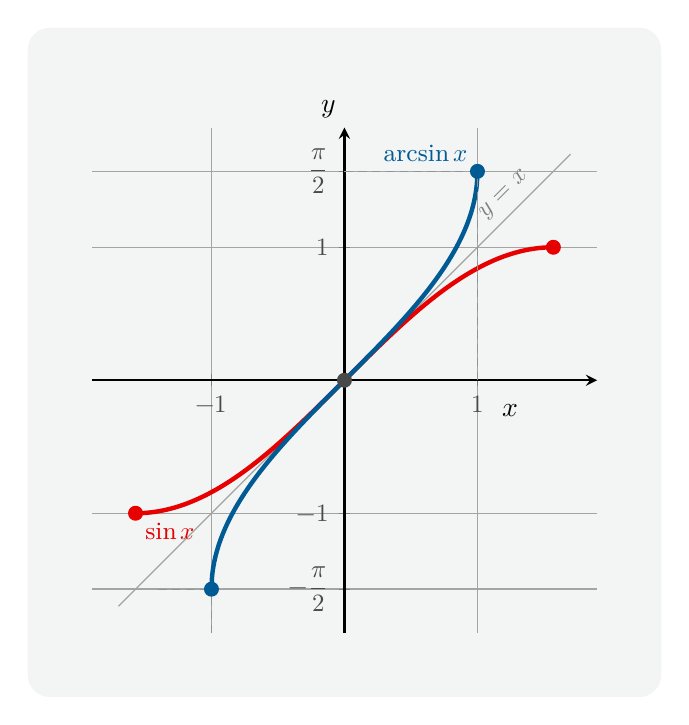
\begin{tikzpicture}[
    show background rectangle,
    background rectangle/.style={fill=my_lightgray, rounded corners=8pt},
    inner frame sep=0.8cm
]

% arcsin(x): domain [-1, 1], range [-π/2, π/2]
% axis equal used: the function maps [-1,1] to [-π/2, π/2] and equal scaling
% correctly represents its geometric relationship to the unit circle.
\begin{axis}[
    axis lines = center,
    xlabel = {$x$},
    ylabel = {$y$},
    xlabel style = {at={(axis cs:1.25,0)}, anchor=north, yshift=-5pt},
    ylabel style = {anchor=south east},
    grid = both,
    grid style = {line width=0.3pt, draw=my_darkgray!30},
    major grid style = {line width=0.5pt, draw=my_darkgray!50},
    axis equal,
    axis line style = {thick},
    xmin = -1.4, xmax = 1.4,
    ymin = -1.9, ymax = 1.9,
    xtick = {-1, 0, 1},
    ytick = {-1.5708, -1, 0, 1, 1.5708},
    yticklabels = {$-\dfrac{\pi}{2}$, $-1$, $0$, $1$, $\dfrac{\pi}{2}$},
    yticklabel style = {font=\small, text=my_darkgray},
    xticklabel style = {font=\small, text=my_darkgray},
    width=8cm, height=8cm,
    clip=false,
]

% Diagonal y = x: mirror axis for the inverse relationship
\addplot[
    draw=my_darkgray!50,
    thin,
    domain=-1.7:1.7
]{ x };
\node[anchor=south, rotate=45, font=\small, text=my_darkgray!70]
    at (axis cs:1.3, 1.3) {$y = x$};

% sin(x) restricted to [-π/2, π/2]: the function being inverted
\addplot[
    draw=my_red,
    samples=300,
    ultra thick,
    domain=-1.5708:1.5708
]{ sin(deg(x)) };

% Closed endpoints of sin on [-π/2, π/2]: (-π/2, -1) and (π/2, 1)
\addplot[
    mark=*,
    mark size=2.5pt,
    only marks,
    draw=my_red,
    fill=my_red
] coordinates {(-1.5708, -1) (1.5708, 1)};

\node[anchor=north west, font=\small, text=my_red]
    at (axis cs:-1.5708, -1) {$\sin x$};

% arcsin(x) on its full closed domain [-1, 1]
\addplot[
    draw=my_darkblue,
    samples=500,
    ultra thick,
    domain=-1:1
]{ asin(x) * pi / 180 };

% Closed endpoints: (-1, -π/2) and (1, π/2)
\addplot[
    mark=*,
    mark size=2.5pt,
    only marks,
    draw=my_darkblue,
    fill=my_darkblue
] coordinates {(-1, -1.5708) (1, 1.5708)};

\node[anchor=south east, font=\small, text=my_darkblue]
    at (axis cs:1, 1.5708) {$\arcsin x$};

% Mark the origin (0, 0), shared by both curves
\addplot[
    mark=*,
    mark size=2.5pt,
    only marks,
    draw=my_darkgray,
    fill=my_darkgray
] coordinates {(0, 0)};

% Dashed reference lines showing domain and range boundaries
\addplot[draw=my_darkgray!60, densely dashed, thin]
    coordinates {(-1, -1.9) (-1, -1.5708)};
\addplot[draw=my_darkgray!60, densely dashed, thin]
    coordinates {(1, 0) (1, 1.5708)};
\addplot[draw=my_darkgray!60, densely dashed, thin]
    coordinates {(-1.4, -1.5708) (-1, -1.5708)};
\addplot[draw=my_darkgray!60, densely dashed, thin]
    coordinates {(0, 1.5708) (1, 1.5708)};

\end{axis}
\end{tikzpicture}
\end{document}
